\subsection*{Definition}

My theory aims to explain the lack of technological spillover from foreign firms to private firms. I define

\begin{itemize}[nosep]
\item \textit{foreign firms} as firms with over 50\% ownership belonging to private foreign individuals, companies, or organizations
\item \textit{private firms} as firms with over 50\% ownership belonging to private domestic individuals, companies, or organizations
\item \textit{state firms} as firms with over 50\% ownership belonging to the host government, \\

and

\item \textit{technological spillover} as the beneficial effects of foreign firms' technological knowledge on the productivity and innovative ability of private firms
\end{itemize}

\subsection*{The argument in three steps}

\begin{enumerate}
\item I argue that for FDI to have a growth enhancing effect, there must be technological spillover from foreign firms to private firms. Therefore, if we see that there is little technological spillover, it must mean that the government is attracting FDI for reasons other than growth.

\item I argue that corruption (i.e. bribes from foreign firms) is one reason (besides growth) that the government wants FDI for. The testable implication is that corruption in a country (sector) is associated with a lack of technological spillover between foreign and private firms in that country (sector). At this step, the level of corruption in a country (sector) is treated as exogenous.

For this argument to be convincing, one must take into account alternative explanations, i.e. reasons besides corruption and growth that governments may want FDI for:
\begin{itemize} 
\item Employment: under strong pressure for employment generation, the government may want FDI purely for the jobs it brings instead of long-term economic growth. To account for this alternative explanation, I will control for the growth rate of the labor force. Since labor force growth is largely determined 18-20 years prior, it is plausibly exogenous to other variables in the current period and thus well-behaved statistically.  
\item Capital: In the early-stage of development, a country may deliberately pursue a capital-driven instead of technology-driven growth. To account for a country's immediate need for capital, I will control for the aggregate capital stock.
\item Election cycle: Much research has shown that the election calendar puts populist pressure on the incumbent government, leading to manipulation of macroeconomic factors such as the exchange rate \citep{Blomberg2001}. Similarly, one may argue that the government attracts FDI to generate positive headlines near election dates even though these FDI projects do not have a large impact on long-term growth. To account for this alternative explanation, I will control for whether a foreign firm establishes in an election year.
\end{itemize}

\item Finally, I endogenize the choice of government officials to engage in corruption by explicitly considering their utility maximization. To get a handle on the options available in the officials' calculus, I hold the political system constant by focusing on the case of Vietnam. With its variation in FDI attraction and private sector development, Vietnam's provinces serve as an insightful microcosm of the cross-national differences. I argue that, in Vietnam, whether FDI creates technological spillover depends on whether provincial officials prefer bribes by foreign firms or promotions by the central government, of which private sector development is an important criterion.
\end{enumerate}

\subsection{Step 1: The growth enhancing effect of FDI depends on technological spillover}

As well-known from neoclassical growth theory, the diminishing return to capital will at one point stop capital from accumulating further, preventing long-run economic growth to be permanently driven by capital accumulation alone \citep{Solow1956}. Therefore, long-run growth ultimately requires technological innovation, which continually increases the productivity of capital and counteracts the diminishing returns.

This insight implies that FDI cannot promote the host country's growth simply from the amount of capital it brings. Therefore, FDI only has a highly uncertain impact on growth and poverty reduction \citep{Nair-Reichert2001, Carkovic2002, Guerra2009}. Scholars have further confirmed that FDI can only a growth-enhancing impact if there is technological spillover from the foreign to the domestic sectors \citep{Nunnenkamp2004}. This empirical finding provides support for \citet{Findlay1978}'s groundbreaking model of FDI and growth, in which technology spillover from foreign firms shift the domestic factor-price frontier to the right, allowing more output from the same input, resulting in higher profits and higher wages (i.e. higher savings) for the domestic sector. This ultimately leads to a continually increasing domestic capital stock.

Since FDI can only be beneficial to growth if there is technological spillover, if one does not observe spillover, it must mean that the host government is attracting FDI for reasons other than growth. In the next step in the theory, I argue that bribe from foreign firms is one such reason.


\subsection{Step 2: FDI and corruption (cross-nationally and cross-sectorally)}

\subsubsection{Defining corruption}

Defining corruption has been a long-standing and inconclusive debate \citep{Johnston1996}. The contention stems from the normative nature of the ``corruption'' concept, which shifts significantly across context and thus difficult to build an analytical edifice upon. 

Consider the most common definition of corruption as ``the abuse of public roles for private gains.'' Make no mistake, this definition is not always clear cut. What constitutes ``abuse''? The term implies the violation of certain standards, which only further asks: what standards are supposed to be adhered to? Some scholars emphasize law-based standards, but the law is not always legitimate \citep[17]{Johnston2004}. Yet others argue for norm-based standards, but difference in norms across societies can be so extensive and unsystematic that renders a cross-country analysis untenable. Indeed, nepotism and cronyism in one society may be social capital in another, with all shades of favoritism in between \citep{Rosen2010}. 

In addition, the distinction between ``public'' and ``private'' are not always clear, especially during rapid economic liberalization and privatization. As the rules change continuously, the dividing line between an innovator and a rule-breaker is but a thread left blowing in the political wind \citep{Sun2004}.

In spite of its shortcomings, the definition of corruption as the ``abuse of public role for private gains'' works well for my research. While this definition may fail as a universal classification of corrupt act, within the scope of my research project its unclarities are largely resolved. First, regarding the unclarity over ``abuse,'' I focus on a law-based definition because of its precision, stability, and broad coverage. The legitimacy of the ``law'' is not as big of a concern because the vast majority of countries with substantial FDI maintain sovereignty over their territory and have laws with a binding impact on their economic life, especially the formal sector in which foreign firms operate. (List the countries in the doing business survey, and whether any of them is a failed state). In addition, a law-based definition fits well with the way corruption is often framed in business surveys, my main source of data, as ``paying informal fees.'' Regardless of whether the respondents think these fees are legitimate or acceptable, it is clear to both the officials and the firms whether these fees are official, as documented in formal laws.

Second, the ``public'' and ``private'' divide is also clear cut within the scope of my project. I focus on corrupt acts in the context of officials exchanging public resources under their control for bribes from foreign firms (e.g., expedited bureaucracy, access to land, harass-free inspections, etc.). It is clear that these public resources and services should be distributed fairly, and that the payments are going to the officials' private wealth instead of the state's coffer.

\subsubsection{The relationship between corruption and FDI}

The majority of literature on the relationship between corruption and FDI focuses on showing that a high level of corruption deters FDI \citep{Wei2000, Hakkala2008, Al-Sadig2009}. (Summarize a bit here) 

But what about foreign firms that choose to invest in a highly corrupt environment nonetheless? One strain of the literature argues that foreign firms can help reduce corruption in host country via regulatory pressure effect, demonstration effect, and professionalization effect \citep{Kwok2006}; or via competing away the rents of the domestic firms, reducing the supply of bribes \citep{Sandholtz2003}. In these works, corruption between the host government and the foreign firm has been conceptualized as \textit{predatory}.

My research offers a new perspective, recognizing that, compared to domestic firms, foreign firms always have the freedom to move out of the country or at least stop bringing in capital. Therefore, the exchange between the government and foreign firms are always more voluntary compared to private firms.\footnote{There is an argument about FDI being harder to relocate, and thus subject to creeping expropriation. However, corruption doesn't tend to change that quickly, and a foreign investor looks into a country knows relatively well the level of corruption that they are getting involved with.} In this angle, corruption between the government and the foreign firm can be \textit{collusive}, with government officials getting bribe and foreign firms getting advantages over domestic firms (e.g. an expedited bureaucracy or privileged use of public resources) \citep{Hellman2002}. Indeed, there are evidence of foreign firms bribing to get an upper hand in the local market\footnote{http://www.nytimes.com/2012/04/22/business/at-wal-mart-in-mexico-a-bribe-inquiry-silenced.html?pagewanted=all} or to pursue rent in protected industries \citep{Malesky2015}. 

Such collusive corruption between the government and foreign firm can be the key to explain the puzzle why governments may want to attract a lot of FDI despite the lack of developmental impact. One may say that (corrupt) institutions matter, but not only to \textit{how much} FDI a country can attract as the literature has studied, but also \textit{which kind}.

\subsubsection{The model of interaction between foreign firms and officials}

The sequencing of the game is as follows:
\begin{enumerate}
\item \textit{At the start of the game, the level of corruption in a country (sector) is given.}

It is reasonable to assume that the level of corruption is exogenously given. High level of corruption in a country may be largely the result of a political system that fails to produce accountability. Such political system is more likely to be the cause than the result of lacking technological spillover. Similarly, high level of corruption in a sector may be largely due to the nature of that sector, e.g. resource-intensive, high fixed cost leading to natural monopoy, etc. which is exogenous.

\textit{If the level of corruption is high, the government is mainly interested in FDI as a source of rent, not as a source of growth.}

 There are several reasons why the government is interested in seeking rent from FDI firms instead of domestic firms. First, if foreign firms are more profitable than domestic firms, they have more rent to be extracted. Second, if foreign firms are larger than domestic firms, they facilitate coordination and allow corruption to be better kept secret among fewer actors. Third, if the interests of firms and the government misalign in the future, foreign firms have both the options of ``exit'' and ``voice,'' whereas domestic firms only have ``voice.'' The government would much prefer an exiting foreign firm to a domestic firm voicing its interest. The first and second reasons also indicate that my theory is most applicable when the entering FDI firms are large.
 
\item \textit{The foreign firm weighs the cost of corruption against the benefits of entering the country (sector), such as natural resource, local market, or cheap labor. If the benefit outweighs the cost, the firm enters the country (sector).}\footnote{\Cref{fig:fdi_corruption} shows that among countries with a lot of FDI, the level of corruption runs the full gamut. This confirms that foreign firms often enter a country despite the cost of corruption.}
\item Since the government brings in the foreign firm for rent, not for long-term growth, we will see less technological spillover in this country (sector).
\end{enumerate}

The theory leads to two testable hypotheses:

\begin{quote}
Hypothesis: The presence of large FDI firms in corrupt countries is associated with a lack of technological spillover in those countries.
\end{quote}

\begin{quote}
Hypothesis: The presence of large FDI firms in corrupt sectors is associated with a lack of technological spillover in those sectors.
\end{quote}

\subsection{Step 3: Endogenizing government officials' decision to engage in corruption with foreign firm}

In the model presented above, the level of corruption is exogenous and deterministically dictates whether government officials attract low-spillover FDI. There is not yet a strategic component in the officials' decision. 

This section endogenizes the decision by government officials to engage in corruption with foreign firm. To get a handle on this question, we need to know the utility calculation of government officials, which in turn requires knowing the options provided to the officials within the country's political economic system. 

Such is a big and difficult question to study with a cross-national design due to an insurmountable degree of endogeneity stemming from unobservable and unmeasurable differences across political systems. Therefore, at this step, I focus on the case of Vietnam, whose sub-national variation in FDI flow and private sector development serve as an excellent testing ground.

In addition to the endogeneity problem, a cross-national study of corruption suffers from well-known conceptual and measurement issues. Conceptually, corruption means different things in different countries \citep{Rosen2010}. Empirically, even if we restrict corruption to a narrow but clear-cut definition, i.e. the act of bribery in exchange to public goods that should be equally available, it is still very difficult to measure corruption well due to sensitivity bias in surveys. Focusing on the case of Vietnam does not only keep constant the locale-dependent definition of corruption but also takes advantage of a survey list experiment conducted by \citet{Malesky2015} to accurately measure the level of corruption across provinces and sectors without sensitivity bias.

\subsubsection{Theory: Corruption with foreign firms as a choice by Vietnamese officials} 

I argue that the key to provincial variation in corruption with foreign firms is the principal-agent relationship between Vietnam's central and the provincial governments. On the one hand, the central government cares more about the spillover effect of FDI and uses promotion to reward local officials that attract high-spillover FDI. On the other hand, local officials have more opportunities to engage in corruption with foreign firms, and should they decide that the private benefit of corruption is greater than that of promotion, they will prioritize foreign firms that bring bribes over those that have high spillover effects.

The reason behind such difference in the preference of central and local governments is the fact that FDI projects are approved and managed at the provincial level. While the central law may be uniform in the book, its implementation varies widely across sub-national units in Vietnam \citep{Meyer2005}.\footnote{Vietnam's sub-national variation in implementation generalizes well to other cases, such as China \citep{Thun2006}} Therefore, the provincial government holds valuable services for sale to foreign firms. In contrast, the central government is more removed from direct contact with FDI firms and thus less likely to benefit from corruption than provincial leaders. 

In addition, the central government is much more concerned with overall economic growth, which is central to the longevity of the regime \citep{Malesky2008}. It wants to attract high-spillover FDI and uses promotion to reward local officials that accomplish this goal. On the other hand, each provincial leader is incentivized to free-ride on the developmental effort of other provinces and of the central to keep the entire regime stable. Therefore, local officials value the spillover effect of FDI only insofar as the opportunities for promotion that it brings.

Fortunately for the central government, the principal-agent problem in this context is partially solved because monitoring is not too difficult. Indeed, the central government can observe the economic performance of the provinces and use personnel management to punish and reward provincial officials \citep{Sheng2007, Li2005}.\footnote{\citet{Shih2012} recently argue that economic performance does not matter to cadre promotion. However, they investigate all members of the Chinese Central Committee, including the central party apparatus, the army, and the central economic bureaucracy. These actors are not the important decision-makers in our theory.} Therefore, the principal-agent problem is only severe when provincial officials are not interested in further promotion to the central government. This suggests that there will be a variation in the level of FDI's spillover effect across provinces according to provincial officials' interest in promotion. 

By looking at this variation in the career interest of provincial officials, my theory contributes a fresh angle to the current literature on the relationship between decentralization and corruption. So far, scholars have only postulated a one-way relationship: either decentralization increases bribery \citep{Fan2009} or reduces it \citep{Guerra2009}. In my model, how decentralization affects corruption is conditional on the local officials' interest in the promotions offered by the central as carrots.

\subsubsection{The model of interaction between the local and central governments}

The game has two players: the central government and the provincial official. The sequencing of the game is as follows:
\begin{enumerate}
\item At the start of the game, the endowment of a province is given.\footnote{The assumption that the endowment is exogenous is reasonable. First, if it is the kind of endowment that cannot be affected by past provincial policies, e.g. natural resources, proximity to market, then it is truly exogenous. Second, even if it is the kind of endowment that can be affected by past policies, e.g. quality of the labor force, infrastructure quality, etc., it is usually good for both foreign and domestic firms. Therefore, at the start of the game, there is not yet any discrimination between foreign and domestic firms.}
\item The provincial official observes his endowment and calculates his current wealth, i.e. the bribes from FDI firms that chose his province due to its endowment.
\item The provincial official calculates the return of pursuing a promotion, which is a ``gamble'' with uncertainty. In this gamble,

the return of pursuing a promotion $=$ the return of the promotion $\times$ the probability of getting the promotion $(p)$.

In addition, $p = p_0 + p_1$, with $p_0$ being the base chance of getting the promotion, and $p_1$ being the added chance if the official decides to develop the domestic sector as the central government desires.

\item The provincial official has to decide between keeping his current wealth (i.e. seek rents from FDI) or gambling (i.e. focus on private sector development to get a $p_0 + p_1$ chance of getting the promotion). Assuming that the official is risk averse, he prefers a small gamble over a large one. In this way, the base chance $p_0$ matters. If $p_0$ is small, it is highly uncertain that the official will get the promotion even with the added $p_1$. Therefore, the official is more likely to seek rent from the foreign firm instead of pursuing a promotion when the base chance $p_0$ is small. 
\end{enumerate}

Three key assumptions in the theory above deserve further examination:
\begin{enumerate}
\item Why wouldn't Vietnam's central government worry that a developed private sector may lead to social change that ultimately undermines its rule?

First, there is a large scholarship showing that authoritarian regimes are very adept at using institutions to manage regime outsiders in general and business in particular \citep{Gandhi2006, Gandhi2008, Wright2008, Le2015}. Second, if the legitimacy of the regime rests heavily on delivering economic growth, then the short-term risk of an economic downturn creating instability features much more prominently than the long-term concern with social changes. Third, it is possible to foster economic growth while restricting political freedom (e.g. Singapore). Indeed, growth can make a regime, both democratic and authoritarian, more stable, and creates room for political control \citep{Przeworski1997}.

\item Why don't provincial leaders seek rent from the domestic sector? 

First, Vietnam's private sector was very small when FDI was first allowed into Vietnam. The size and the profitability of the average domestic firm is still smaller than those of foreign firms today. Therefore, there are both fewer rents and more coordination problems if provincial officials want to seek rents from domestic firms. Second, ironically, if officials want to grow the private sector for future rent-seeking, they must promote an enabling business environment that are free from rent-seeking. In contrast, engaging in corruption with large and existing FDI firms is much more convenient. Essentially, corrupt provincial officials have shifted the cost of building a thriving domestic sectors to the home countries of FDI firms and now extract rents from the high productivity and high profitability of these firms. 

\item Is it reasonable to frame seeking rents and seeking technological spillover from FDI as a dichotomous choice for provincial officials?

In the above model, provincial officials have to choose between attracting FDI for spillover or for bribes. One may argue that this trade off does not exist. Indeed, if the fact that a foreign firm engages in corruption does not affect its level of spillover, then even if provincial officials prioritize FDI for rents it would not have any effect on the level of spillover.

However, the trade off does exist. This is because, in exchange for bribes, provincial officials must offer some advantages over domestic firms to foreign firms. This can be lower tax rate, easier access to land, more attention to concerns of firms, etc. Without efforts by the local government to nurture the private sector, it is unlikely that private firms have the necessary sophistication to engage in contracts with foreign firms or to imitate foreign firms' technology.

\Cref{fig:fdi_bias_vietnam} provides evidence that when provincial officials are biased towards foreign firms, private firms are poorly supported. The x-axis shows how helpful the province is according to private firms. The y-axis shows the fairness of provincial officials in treating foreign and private firms (as perceived by private firms). The graph shows that if a province is biased towards foreign firms, it will also treat private firms poorly (the lower-left quadrant). The relationship is even stronger among provinces with a lot of FDI (blue labels and line).
\end{enumerate}

\begin{figure}[!ht]
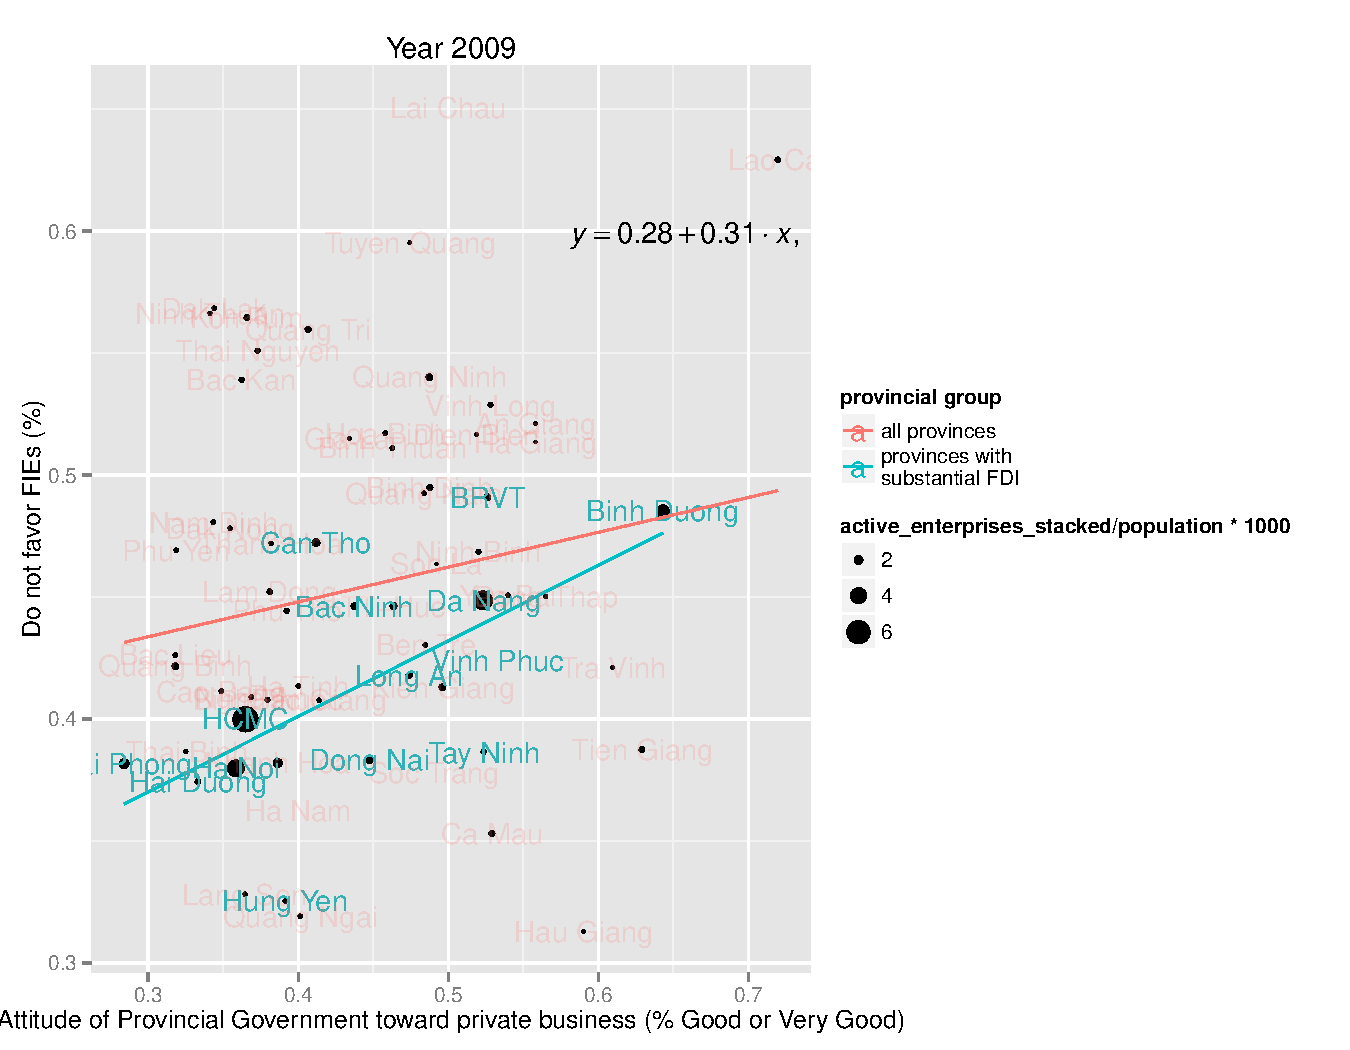
\includegraphics[width=\textwidth,keepaspectratio]{../figure/FDI_bias}
\caption{The relationship between a province's FDI bias and attitude towards the private sector}
\label{fig:fdi_bias_vietnam}
\end{figure}

In sum, I propose a hypothesis about variation across Vietnam's provinces:

\begin{quote}
Hypothesis: The presence of large FDI firms in provinces whose leaders are not interested in promotion is associated with a low level of spillover effect.
\end{quote}
